% 최소 컴파일 하네스 — FO3 그림 조각 검증 전용 (문서 원본과 무관).
% 빌드: xelatex -interaction=nonstopmode _harness.tex  (오류 0 확인용)
% ch1+ch2 preamble 의 tikz 라이브러리 합집합 + 사용 매크로만 정의.
\documentclass[11pt,a4paper]{article}
\usepackage[margin=18mm]{geometry}
\usepackage{kotex}
\usepackage{amsmath,amssymb,mathtools,bm}
\usepackage{graphicx}
\usepackage{tikz}
\usetikzlibrary{positioning,arrows.meta,calc,fit,backgrounds,decorations.pathreplacing}
% --- 사용 매크로(양 preamble 에서 발췌) ---
\newcommand{\dd}{\mathrm{d}}
\newcommand{\eq}{\mathrm{eq}}
\newcommand{\app}{\mathrm{app}}
\newcommand{\cell}{\mathrm{cell}}
\newcommand{\bg}{\mathrm{bg}}
\newcommand{\rxn}{\mathrm{rxn}}
\newcommand{\hys}{\mathrm{hys}}
\newcommand{\oc}{\mathrm{oc}}
\newcommand{\rev}{\mathrm{rev}}
\newcommand{\config}{\mathrm{config}}
\newcommand{\vib}{\mathrm{vib}}
\newcommand{\dis}{\mathrm{dis}}
\newcommand{\chg}{\mathrm{chg}}
\newcommand{\kB}{k_{\mathrm B}}
\begin{document}
\begin{center}\large FO3 그림 조각 컴파일 검증 하네스\end{center}
% ====================================================================
% CAND-FO3-1 : 합성 관측 dQ/dV = C_bg + sum_j Q_j xi_eq(1-xi_eq)/w_j  (N9, eq:sum)
%   배치 제안: §10 (sec:sum) 식~(eq:sum) 박스 직후. fig:staging(분리 peak)의 짝 그림.
%   좌표 = 식 그대로의 수치 평가. fig:staging 과 동일한 tab:staging 초기값
%     (U={0.210,0.140,0.120,0.085} V, w={0.020,0.016,0.014,0.012} V, Q={0.10,0.12,0.25,0.50} Q_cell),
%     방전 sigma_d=+1, 배경 C_bg=0.6 Q_cell/V(예시 상수). python 평가·하드코딩.
%   사용 라이브러리: arrows.meta (ch1 preamble 에 로드됨).
% ====================================================================
\begin{figure}[t]
\centering
\begin{tikzpicture}[x=38cm,y=0.36cm,>=Latex]
% ---- axes ----
\draw[-{Latex[length=1.6mm]}] (0.028,0) -- (0.268,0) node[below,font=\scriptsize] {$V_n$ [V]};
\draw[-{Latex[length=1.4mm]}] (0.028,0) -- (0.028,13.4) node[above,font=\scriptsize,align=center] {$\dd Q/\dd V$\\{\tiny[$Q_\cell/$V]}};
\foreach \vv in {0.05,0.10,0.15,0.20,0.25} {\draw (\vv,0.18)--(\vv,-0.18) node[below,font=\scriptsize] {\vv};}
\foreach \yy in {4,8,12} {\draw (0.0268,\yy)--(0.0292,\yy) node[left,font=\scriptsize] {\yy};}
% ---- background pedestal C_bg (dotted horizontal) ----
\draw[densely dotted] (0.030,0.6) -- (0.260,0.6);
\node[font=\tiny,anchor=west] at (0.212,0.42) {$C_\bg$ (예시 상수)};
% ---- four individual transition contributions (thin gray, +C_bg baseline) ----
\draw[black!45,thin] plot[smooth] coordinates {(0.1100,0.6332) (0.1152,0.6429) (0.1203,0.6553) (0.1255,0.6711) (0.1307,0.6913) (0.1359,0.7170) (0.1410,0.7494) (0.1462,0.7900) (0.1514,0.8404) (0.1566,0.9022) (0.1617,0.9769) (0.1669,1.0653) (0.1721,1.1673) (0.1772,1.2813) (0.1824,1.4034) (0.1876,1.5271) (0.1928,1.6438) (0.1979,1.7428) (0.2031,1.8136) (0.2083,1.8477) (0.2134,1.8408) (0.2186,1.7937) (0.2238,1.7124) (0.2290,1.6063) (0.2341,1.4862) (0.2393,1.3621) (0.2445,1.2422) (0.2497,1.1319) (0.2548,1.0343) (0.2600,0.9505)};
\draw[black!45,thin] plot[smooth] coordinates {(0.0600,0.6499) (0.0655,0.6700) (0.0710,0.6981) (0.0766,0.7369) (0.0821,0.7904) (0.0876,0.8631) (0.0931,0.9606) (0.0986,1.0885) (0.1041,1.2515) (0.1097,1.4510) (0.1152,1.6820) (0.1207,1.9293) (0.1262,2.1657) (0.1317,2.3550) (0.1372,2.4611) (0.1428,2.4611) (0.1483,2.3550) (0.1538,2.1657) (0.1593,1.9293) (0.1648,1.6820) (0.1703,1.4510) (0.1759,1.2515) (0.1814,1.0885) (0.1869,0.9606) (0.1924,0.8631) (0.1979,0.7904) (0.2034,0.7369) (0.2090,0.6981) (0.2145,0.6700) (0.2200,0.6499)};
\draw[black!45,thin] plot[smooth] coordinates {(0.0500,0.7187) (0.0548,0.7667) (0.0597,0.8335) (0.0645,0.9261) (0.0693,1.0533) (0.0741,1.2265) (0.0790,1.4585) (0.0838,1.7630) (0.0886,2.1511) (0.0934,2.6262) (0.0983,3.1762) (0.1031,3.7649) (0.1079,4.3277) (0.1128,4.7785) (0.1176,5.0313) (0.1224,5.0313) (0.1272,4.7785) (0.1321,4.3277) (0.1369,3.7649) (0.1417,3.1762) (0.1466,2.6262) (0.1514,2.1511) (0.1562,1.7630) (0.1610,1.4585) (0.1659,1.2265) (0.1707,1.0533) (0.1755,0.9261) (0.1803,0.8335) (0.1852,0.7667) (0.1900,0.7187)};
\draw[black!45,thin] plot[smooth] coordinates {(0.0300,1.0173) (0.0340,1.1761) (0.0379,1.3930) (0.0419,1.6870) (0.0459,2.0814) (0.0498,2.6032) (0.0538,3.2803) (0.0578,4.1359) (0.0617,5.1787) (0.0657,6.3880) (0.0697,7.6977) (0.0736,8.9859) (0.0776,10.0826) (0.0816,10.8046) (0.0855,11.0118) (0.0895,10.6615) (0.0934,9.8255) (0.0974,8.6608) (0.1014,7.3521) (0.1053,6.0592) (0.1093,4.8891) (0.1133,3.8946) (0.1172,3.0872) (0.1212,2.4532) (0.1252,1.9674) (0.1291,1.6016) (0.1331,1.3299) (0.1371,1.1298) (0.1410,0.9835) (0.1450,0.8770)};
% ---- composite total (thick) ----
\draw[very thick] plot[smooth] coordinates {(0.0300,1.0544) (0.0340,1.2284) (0.0381,1.4666) (0.0421,1.7905) (0.0461,2.2264) (0.0502,2.8050) (0.0542,3.5582) (0.0582,4.5129) (0.0623,5.6799) (0.0663,7.0376) (0.0704,8.5146) (0.0744,9.9809) (0.0784,11.2606) (0.0825,12.1745) (0.0865,12.6029) (0.0905,12.5361) (0.0946,12.0777) (0.0986,11.3989) (0.1026,10.6696) (0.1067,10.0060) (0.1107,9.4520) (0.1147,8.9908) (0.1188,8.5730) (0.1228,8.1460) (0.1268,7.6747) (0.1309,7.1479) (0.1349,6.5750) (0.1389,5.9767) (0.1430,5.3765) (0.1470,4.7962) (0.1511,4.2535) (0.1551,3.7621) (0.1591,3.3312) (0.1632,2.9661) (0.1672,2.6682) (0.1712,2.4352) (0.1753,2.2622) (0.1793,2.1420) (0.1833,2.0659) (0.1874,2.0242) (0.1914,2.0068) (0.1954,2.0036) (0.1995,2.0048) (0.2035,2.0018) (0.2075,1.9880) (0.2116,1.9585) (0.2156,1.9111) (0.2196,1.8460) (0.2237,1.7654) (0.2277,1.6729) (0.2318,1.5730) (0.2358,1.4700) (0.2398,1.3680) (0.2439,1.2702) (0.2479,1.1789) (0.2519,1.0956) (0.2560,1.0211) (0.2600,0.9555)};
% ---- transition labels (at each individual peak) ----
\node[font=\tiny,black!55,anchor=south east] at (0.0800,11.15) {$2\!\to\!1$};
\node[font=\tiny,black!55,anchor=west] at (0.1230,5.10) {$2\mathrm L\!\to\!2$};
\node[font=\tiny,black!55,anchor=south west] at (0.1400,2.50) {$3\!\to\!2\mathrm L$};
\node[font=\tiny,black!55,anchor=south] at (0.2083,1.90) {$4\!\to\!3$};
% ---- overlap annotation ----
\draw[->,gray] (0.1150,9.0) -- (0.1010,10.3);
\node[font=\tiny,gray,anchor=west,align=left] at (0.1150,8.6) {겹침 shoulder\\($2\!\to\!1{+}2\mathrm L\!\to\!2$)};
\node[font=\scriptsize,anchor=west] at (0.1120,12.20) {합성(관측) $=$ 굵은 실선};
% ---- discharge direction ----
\draw[->,semithick] (0.150,12.6) -- (0.230,12.6);
\node[font=\tiny,anchor=south] at (0.190,12.6) {방전(탈리튬화) $\xi\!\uparrow$};
\end{tikzpicture}
\caption{합산 노드(N9)가 내는 \emph{관측} $\dd Q/\dd V$ 곡선 --- 배경과 네 전이 봉우리의 선형 합(식~\eqref{eq:sum};
좌표는 식 그대로의 수치 평가). 얇은 회색은 전이별 기여 $Q_j\,\xi_\eq(1-\xi_\eq)/w_j$(식~\eqref{eq:eqpeak}),
굵은 실선은 그 합에 배경을 얹은 합성 곡선이며, 이 굵은 실선이 실제 측정되는 한 곡선이다. 입력은
그림~\ref{fig:staging} 과 같은 표~\ref{tab:staging} 초기값($U_j{=}0.210/0.140/0.120/0.085$ V,
$w_j{=}0.020/0.016/0.014/0.012$ V, $Q_j{=}0.10/0.12/0.25/0.50\,Q_\cell$, 방전 $\sigma_d{=}{+}1$)이고,
배경 $C_\bg$ 는 예시 상수 pedestal($0.6\,Q_\cell/$V --- 모델 입력으로 상수 또는 $V$ 함수)이다. 그림~\ref{fig:staging}
이 네 봉우리를 \emph{분리}해 보였다면, 이 그림은 그것들이 배경 위에서 \emph{합쳐진} 모습을 보인다 --- 중심이
가까운 $2\!\to\!1\cdot2\mathrm L\!\to\!2$ 가 한 봉우리로 겹쳐(shoulder) 서론의 ``peak 겹침'' 관측을 그대로
드러내고, 멀리 떨어진 $4\!\to\!3$ 만 별개 봉우리로 남는다. 순높이는 전이마다 $Q_j/(4w_j)$ 로 크게 달라
($2\!\to\!1$ 이 지배) 합성 곡선의 모양을 $2\!\to\!1$ 봉우리가 이끈다.}
\label{fig:cand-fo3-1}
\end{figure}

\clearpage
% ====================================================================
% CAND-FO3-2 : 가역 발열의 SOC 부호 교대  q_rev/I(x_bar) = -T dU_oc/dT  (eq:qrev)
%   배치 제안: §2.8 (sec:synthesis) 표~(tab:qrev) 직후/직전.
%   좌표 = 식 그대로의 수치 평가: 음함수 sum_j Q_j xi_eq,j(U_oc,T)=Q x_bar (eq:implicit)
%     를 x_bar 마다 풀어 U_oc, 중앙차분 dU_oc/dT, q_rev/I=-T dU_oc/dT. n_j=1(w=RT/F), 298.15 K.
%     Chapter 1 4-전이 staging 파라미터. python 평가. 5개 점 표는 tab:qrev 와 정확 일치 검증.
%   ch2 preamble 라이브러리(arrows.meta)만 사용 — 음영은 그리기 순서(fill 먼저)로 backgrounds 불요.
% ====================================================================
\begin{figure}[t]
\centering
\begin{tikzpicture}[x=8.6cm,y=0.023cm,>=Latex]
% ---- region shading (drawn first so it sits behind) ----
\fill[black!5]  (0.02,-102) rectangle (0.680,116);
\fill[black!12] (0.680,-102) rectangle (0.98,116);
% ---- zero line (q_rev = 0) ----
\draw[densely dashed,black!55] (0.02,0) -- (0.98,0);
% ---- axes ----
\draw[-{Latex[length=1.6mm]}] (0.02,-102) -- (0.02,118) node[above,font=\scriptsize,align=center] {$\dot Q_\rev/I$ [mV]\\{\tiny($+$ 발열)}};
\draw[-{Latex[length=1.6mm]}] (0.02,0) -- (0.98,0) node[below=6pt,font=\scriptsize] {$\bar x$ (탈리튬화 분율)};
\foreach \yy in {-100,-50,50,100} {\draw (0.012,\yy)--(0.028,\yy) node[left,font=\scriptsize] {\yy};}
\foreach \xx in {0.2,0.4,0.6,0.8,1.0} {\draw (\xx,4)--(\xx,-4) node[below,font=\scriptsize] {\xx};}
% ---- smooth q_rev/I curve ----
\draw[very thick] plot[smooth] coordinates {(0.050,111.420) (0.070,101.772) (0.091,94.363) (0.111,88.266) (0.132,83.027) (0.152,78.389) (0.173,74.191) (0.193,70.329) (0.214,66.728) (0.234,63.332) (0.255,60.102) (0.275,57.005) (0.295,54.014) (0.316,51.110) (0.336,48.275) (0.357,45.494) (0.377,42.753) (0.398,40.041) (0.418,37.348) (0.439,34.664) (0.459,31.979) (0.480,29.284) (0.500,26.571) (0.520,23.829) (0.541,21.048) (0.561,18.218) (0.582,15.328) (0.602,12.362) (0.623,9.307) (0.643,6.144) (0.664,2.850) (0.684,-0.601) (0.705,-4.242) (0.725,-8.115) (0.745,-12.275) (0.766,-16.791) (0.786,-21.757) (0.807,-27.296) (0.827,-33.569) (0.848,-40.779) (0.868,-49.153) (0.889,-58.890) (0.909,-70.103) (0.930,-82.883) (0.950,-97.717)};
% ---- exact tab:qrev markers ----
\foreach \xb/\qq in {0.10/91.5, 0.25/60.8, 0.50/26.6, 0.75/-13.2, 0.90/-64.9} {
  \fill (\xb,\qq) circle (1.6pt);}
\node[font=\tiny,anchor=south west] at (0.11,91.5) {$(0.10,{+}91.5)$};
\node[font=\tiny,anchor=south west] at (0.26,60.8) {$(0.25,{+}60.8)$};
\node[font=\tiny,anchor=south west] at (0.51,26.6) {$(0.50,{+}26.6)$};
\node[font=\tiny,anchor=north west] at (0.76,-13.2) {$(0.75,{-}13.2)$};
\node[font=\tiny,anchor=north east] at (0.885,-64.9) {$(0.90,{-}64.9)$};
% ---- zero-crossing marker ----
\draw[densely dotted] (0.680,0) -- (0.680,-30);
\fill (0.680,0) circle (1.3pt);
\node[font=\tiny,anchor=north] at (0.680,-32) {부호 반전 $\bar x{\approx}0.68$};
% ---- region labels ----
\node[font=\scriptsize,align=center] at (0.34,102) {방전 \textbf{발열}\\($\dot Q_\rev{>}0$, $\Delta S{<}0$)};
\node[font=\scriptsize,align=center] at (0.85,102) {방전 \textbf{흡열}\\($\dot Q_\rev{<}0$, $\Delta S{>}0$)};
\end{tikzpicture}
\caption{한 종합식이 SOC 축을 따라 스스로 뒤집는 가역 발열의 부호(식~\eqref{eq:qrev}
$\dot Q_\rev/I=-T\,\partial U_\oc/\partial T$; 좌표는 식 그대로의 수치 평가). 각 탈리튬화 분율 $\bar x$ 에서 전하
보존 음함수~\eqref{eq:implicit} 를 풀어 $U_\oc$ 를 얻고, $T{=}298.15$ K 중앙차분으로 $\partial U_\oc/\partial T$ 를
계산한 완전식 결과다(Chapter 1 4-전이 staging, $w_j{=}RT/F$). 점은 표~\ref{tab:qrev} 의 다섯 값과 정확히 일치한다.
저-$\bar x$(Li-rich, stage $2\!\to\!1$ 의 큰 음의 $\Delta S$)에서는 방전이 \emph{발열}($\dot Q_\rev{>}0$)이고,
고-$\bar x$(Li-poor, config 분포 항의 양의 발산)에서는 방전이 \emph{흡열}로 돌아, 부호가 $\bar x{\approx}0.68$
에서 반전한다. 외부 스위치나 임의 함수 없이 세 분포의 가중 합만으로 흡$\cdot$발열 교대가 나온다는 것이 이 곡선의
요지다. 행별 흡$\cdot$발열 판정은 폭의 열적 서식 $w_j{=}n_jRT/F$ 를 전제한 값이며, 지배 두-상 전이의 실측 폭이
$T$-동결에 가까우면 경계 $\bar x$ 가 이동할 수 있다(표~\ref{tab:qrev} 한정과 동일).}
\label{fig:cand-fo3-2}
\end{figure}

\clearpage
% ====================================================================
% CAND-FO3-3 : 단일 평형 peak 의 해부 — eq:eqpeak 한 식에서 읽는 세 양 + FWHM
%   배치 제안: §6 (sec:eqpeak) 식~(eq:eqpeak) 박스 직후.
%   좌표 = 식 그대로의 수치 평가: 종 y=xi(1-xi), xi=logistic[(V-U^d)/w]; 가로축은 w_j 단위.
%     정점 1/4 @중심, 반높이(1/8) 반폭 = ln(1+sqrt2)*2 = 1.7627 w -> FWHM=3.5255 w. python 평가.
%   사용 라이브러리: arrows.meta (ch1 preamble).
% ====================================================================
\begin{figure}[t]
\centering
\begin{tikzpicture}[x=0.95cm,y=13cm,>=Latex]
% ---- shaded area under the bell = Q_j ----
\fill[black!8] plot[smooth] coordinates {(-5.000,0.0066) (-4.494,0.0109) (-3.987,0.0179) (-3.481,0.0290) (-2.975,0.0462) (-2.468,0.0720) (-1.962,0.1081) (-1.456,0.1534) (-0.949,0.2012) (-0.443,0.2381) (-0.063,0.2497) (0.063,0.2497) (0.443,0.2381) (0.949,0.2012) (1.456,0.1534) (1.962,0.1081) (2.468,0.0720) (2.975,0.0462) (3.481,0.0290) (3.987,0.0179) (4.494,0.0109) (5.000,0.0066)} -- (5.0,0) -- (-5.0,0) -- cycle;
% ---- axes ----
\draw[-{Latex[length=1.6mm]}] (-5.4,0) -- (5.6,0) node[below,font=\scriptsize] {$(V-U_j^{\,d})/w_j$};
\draw[-{Latex[length=1.4mm]}] (-5.4,0) -- (-5.4,0.295) node[above,font=\scriptsize] {$\dd Q/\dd V$};
\foreach \xx in {-4,-2,0,2,4} {\draw (\xx,0.006)--(\xx,-0.006) node[below,font=\scriptsize] {\xx};}
% ---- peak-height guide (net height = Q_j/4w_j) ----
\draw[densely dashed] (-5.4,0.25) -- (0,0.25);
\node[font=\scriptsize,anchor=west] at (0.15,0.263) {순높이 $=Q_j/(4w_j)$};
\fill (0,0.25) circle (1.4pt);
% ---- half-maximum + FWHM ----
\draw[densely dotted,black!55] (-5.4,0.125) -- (4.2,0.125);
\draw[{Latex[length=1.2mm]}-{Latex[length=1.2mm]}] (-1.7627,0.125) -- (1.7627,0.125);
\node[font=\scriptsize,fill=black!8,inner sep=1pt] at (0,0.125) {FWHM $=2\ln(3{+}2\sqrt2)\,w_j\approx3.53\,w_j$};
% ---- the bell (thick) ----
\draw[very thick] plot[smooth] coordinates {(-5.000,0.0066) (-4.620,0.0097) (-4.241,0.0140) (-3.861,0.0202) (-3.481,0.0290) (-3.101,0.0412) (-2.722,0.0579) (-2.342,0.0800) (-1.962,0.1081) (-1.582,0.1414) (-1.203,0.1777) (-0.823,0.2120) (-0.443,0.2381) (-0.190,0.2478) (0.063,0.2497) (0.316,0.2438) (0.570,0.2308) (0.823,0.2120) (1.203,0.1777) (1.582,0.1414) (1.962,0.1081) (2.342,0.0800) (2.722,0.0579) (3.101,0.0412) (3.481,0.0290) (3.861,0.0202) (4.241,0.0140) (4.620,0.0097) (5.000,0.0066)};
% ---- center (position) marker ----
\draw[densely dotted] (0,0) -- (0,0.25);
\node[font=\scriptsize,anchor=north] at (0,-0.018) {위치 $=U_j^{\,d}$};
% ---- area label ----
\node[font=\scriptsize,align=center] at (-2.5,0.055) {면적 $=Q_j$\\{\footnotesize $\displaystyle\int\!\dd\xi{=}1$}};
% ---- species label ----
\node[font=\scriptsize,anchor=west,align=left] at (1.9,0.20) {평형 종\\$Q_j\dfrac{\xi_\eq(1{-}\xi_\eq)}{w_j}$};
\end{tikzpicture}
\caption{평형 peak(식~\eqref{eq:eqpeak}) 한 식에서 읽히는 세 양의 해부(좌표는 식 그대로의 수치 평가: 종
$\xi_\eq(1-\xi_\eq)$, $\xi_\eq{=}\mathrm{logistic}[(V-U_j^{\,d})/w_j]$, 가로축은 폭 $w_j$ 단위). \emph{위치}는 분기
중심 $U_j^{\,d}$(정점, $\xi_\eq{=}\tfrac12$), \emph{순높이}는 $Q_j/(4w_j)$($\xi(1-\xi)$ 가 중심에서 $\tfrac14$),
\emph{배경 차감 면적}은 $Q_j$($\int_0^1\dd\xi{=}1$ 이라 종의 적분이 $1$, 음영)이다 --- 세 양이 한 식에서 곧바로
나온다. 반높이 전폭은 $\mathrm{FWHM}=2\ln(3+2\sqrt2)\,w_j\approx3.53\,w_j$ 로 폭 $w_j$ 에 비례한다($n_j{=}1$,
$298$ K 에서 $\approx91$ mV). 종은 $\xi(1-\xi)\ge0$ 이라 양수이고 방향 불변이며, 이 그림은 동역학 꼬리가 폭에
비해 작을 때($L_V\!\to\!0$)의 저전류 기준선이다.}
\label{fig:cand-fo3-3}
\end{figure}

\clearpage
% ====================================================================
% CAND-FO3-4 : 평형 중심의 온도 의존 U_j(T)=(-dH_rxn+T dS_rxn)/F  (eq:Uj), 기울기 dS_rxn/F
%   배치 제안: §3 (sec:center) 식~(eq:Uj) 박스 직후(현재 §3 에 그림 0).
%   좌표 = 식 그대로의 수치 평가: tab:staging 의 (dH_rxn,dS_rxn) 4전이, T=268..328 K. python 평가.
%     기울기 dS/F = +0.301/0.000/-0.052/-0.166 mV/K (전이별 부호 상이).
%   사용 라이브러리: arrows.meta (ch1 preamble).
% ====================================================================
\begin{figure}[t]
\centering
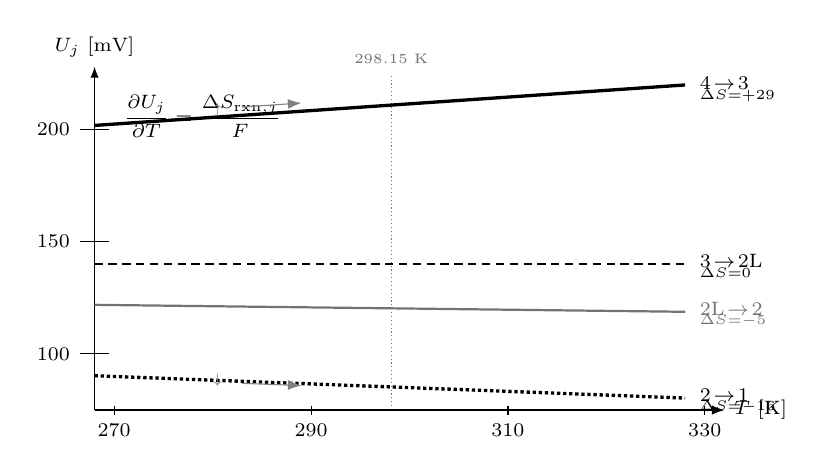
\begin{tikzpicture}[x=0.125cm,y=0.0285cm,>=Latex]
% ---- reference isotherm T=298.15 ----
\draw[densely dotted,black!55] (298.15,75) -- (298.15,225);
\node[font=\tiny,black!55,anchor=south] at (298.15,225) {$298.15$ K};
% ---- axes (y starts at 75 mV; note the offset) ----
\draw[-{Latex[length=1.6mm]}] (268,75) -- (332,75) node[right,font=\scriptsize] {$T$ [K]};
\draw[-{Latex[length=1.4mm]}] (268,75) -- (268,228) node[above,font=\scriptsize] {$U_j$ [mV]};
\foreach \tt in {270,290,310,330} {\draw (\tt,77)--(\tt,73) node[below,font=\scriptsize] {\tt};}
\foreach \uu in {100,150,200} {\draw (269.5,\uu)--(266.5,\uu) node[left,font=\scriptsize] {\uu};}
% ---- four center lines U_j(T) (straight; slope = dS_rxn/F) ----
% 4->3  dS=+29.0  (rises)
\draw[very thick] (268,201.81) -- (328,219.85);
\node[font=\scriptsize,anchor=west] at (328.5,220.5) {$4\!\to\!3$};
\node[font=\tiny,anchor=west] at (328.5,215.0) {$\Delta S{=}{+}29$};
% 3->2L dS=0  (flat)
\draw[thick,densely dashed] (268,139.92) -- (328,139.92);
\node[font=\scriptsize,anchor=west] at (328.5,141.5) {$3\!\to\!2\mathrm L$};
\node[font=\tiny,anchor=west] at (328.5,136.0) {$\Delta S{=}0$};
% 2L->2 dS=-5 (slight fall)
\draw[thick,black!55] (268,121.88) -- (328,118.77);
\node[font=\scriptsize,anchor=west,black!55] at (328.5,120.0) {$2\mathrm L\!\to\!2$};
\node[font=\tiny,anchor=west,black!55] at (328.5,114.5) {$\Delta S{=}{-}5$};
% 2->1 dS=-16 (falls)
\draw[very thick,densely dotted] (268,90.29) -- (328,80.34);
\node[font=\scriptsize,anchor=west] at (328.5,81.5) {$2\!\to\!1$};
\node[font=\tiny,anchor=west] at (328.5,76.5) {$\Delta S{=}{-}16$};
% ---- slope annotation ----
\node[font=\scriptsize,anchor=south west,align=left] at (270,192)
  {$\dfrac{\partial U_j}{\partial T}=\dfrac{\Delta S_{\rxn,j}}{F}$};
% slope-direction arrows
\draw[->,gray] (283,210.0) -- (289,211.8);   \node[font=\tiny,gray] at (280.5,208.5) {$\uparrow$};
\draw[->,gray] (283,86.9) -- (289,85.9);      \node[font=\tiny,gray] at (280.5,88.4) {$\downarrow$};
\end{tikzpicture}
\caption{평형 중심의 온도 의존 $U_j(T)$(식~\eqref{eq:Uj}; 좌표는 식 그대로의 수치 평가: 표~\ref{tab:staging}
의 네 전이 $(\Delta H_{\rxn,j},\Delta S_{\rxn,j})$, $T{=}268$--$328$ K). 각 직선의 기울기가 정확히
$\partial U_j/\partial T=\Delta S_{\rxn,j}/F$ 라, 반응 엔트로피의 \emph{부호}가 중심의 이동 방향을 정한다 ---
$\Delta S{>}0$ 인 $4\!\to\!3$($+29$)은 온도가 오르면 중심이 \emph{올라가고}, $\Delta S{=}0$ 인 $3\!\to\!2\mathrm L$
은 평평하며, $\Delta S{<}0$ 인 $2\!\to\!1$($-16$)$\cdot$$2\mathrm L\!\to\!2$($-5$)은 \emph{내려간다}. 기울기 규모는
$|\Delta S|/F\sim$ 수십 $\mu$V/K$\sim$수십분의 mV/K 이라 $60$ K 창에서 중심이 수$\sim$수십 mV 이동한다 ---
다온도 피팅에서 온도마다 $U_j(T)$ 를 따로 읽어야 하는 까닭이 이 서로 다른 기울기다. 세로축은 $75$ mV 에서
끊어 그렸다.}
\label{fig:cand-fo3-4}
\end{figure}

\end{document}
